\section{Practice Problems}
\begin{enumerate}
    \item Find the region of operation for the following transistors. You may use $V_{tn} = 0.9$V and $\mid V_{tp} = 1$V. The operation condition of NMOS is also shown. PMOS is conducted by holes which is opposite to NMOS so the voltage polarity is different.
    \begin{figure}[H]
        \centering
        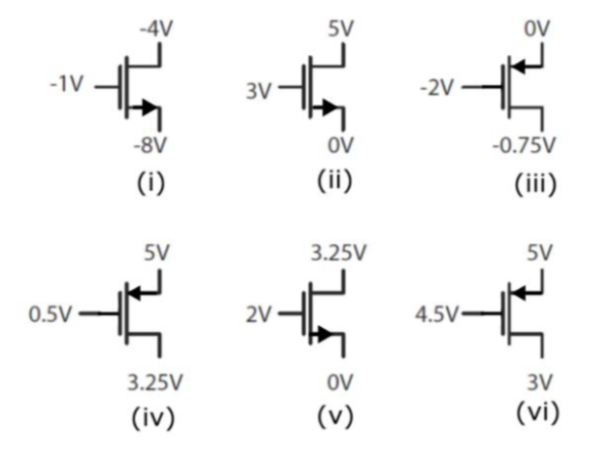
\includegraphics[scale=0.8]{figs/ch05/pp_transistor1.png}
    \end{figure}
    \begin{center}
        \begin{tabular}{|c|c|c|}
            \hline
            Region of operation & Condsitions & \ids \\
            \hline
            Cut-off & \vgs < $V_T$ & \ids $\sim$ 0A \\
            \hline
            Linear/Triode & $V_{GS}$ > $V_T$, $V_{DS} < V_{GS} - V_T$ & \ids = {\large $\frac{W}{L} \mu_n C_{ox} (V_{GS} - V_T - \frac{V_{DS}}{2}) V_{DS}$} \\ [10pt]
            \hline
            Saturation: & $V_{GS}$ > $V_T$, $V_{DS} > V_{GS} - V_T$ & {\large \ids = $\frac{W}{L} \frac{\mu_n C_{ox}}{2} (V_{GS} - V_T)^2 (1+ \lambda V_{DS})$} \\
            \hline
        \end{tabular}
    \end{center}
    \textcolor{blue}{
    \begin{enumerate}
        \item We identify this transistor as a NMOS transistor due to the direction of the arrow. In a NMOS transistor, current flows from drain to source due to electrons being the charge carriers in the NMOS transistor. \vgs = $v_G - v_S$ = 7V and \vds = $v_D - v_S = -4 -(-8) - 4$V. This transistor is in the linear/triode region. 
        \item \vgs = 3V and \vds = 5V. This transistor is in the saturation region.
        \item This is a PMOS transistor. In a PMOS transistor, current flows from source to drain. $|v_{GS}|= 2$V and $|v_{DS}|= 0.75$V. This is in the linear/triode region.
        \item $|v_{GS}| = 4.5$V and $|v_{DS}| = |3.25 - 5| = 1.75$V. This is in the linear/triode region.
        \item $v_{GS} = 2$V and $v_{DS} = 3.25-0 = 3.25$V. This is in the saturation region.
        \item $|v_{GS}| = |4.5-5| = 0.5$V. This is in the cutoff region.
    \end{enumerate}
    }

    \item An ideal $N$-channel MOSFET has the following parameters: $W = 100$ \mun, $L = 1$ \mun, $t_{ox} = 15$ nm, the oxide relative permittivity is 4, the silicon relative permittivity is 12, $N_A = 10^{15}$\conc, $n_i = 10^{10}$\conc, $V_{FB} = -0.2$ V, $\mu_n = 300$\mobility at 300K. $\lambda = 0$.
    \begin{enumerate}
        \item Find the threshold voltage.
        \begin{Ans}
            Threshold voltage is given by the following formula:
            \begin{align*}
                \phi_B &= \frac{kT}{q} \ln\frac{N_A}{n_i} = 0.026 V \ln(\frac{10^{15} \mathrm{ cm}^{-3}}{10^{10} \mathrm{ cm}^{-3}}) = 0.2993 \dots V \\
                C_{ox} &= \frac{\epsilon_{ox}}{t_{ox}} = \frac{4(8.854 \times 10^{-14} \mathrm{F/cm})}{15 \mathrm{nm}} = 3.54 \times 10^{-7} \mathrm{F/cm}^2 \\
                V_t &= V_{FB} + 2\phi_B + \frac{\sqrt{2q\epsilon_s N_A 2 \phi_B}}{C_{ox}} \\
                &= -0.2 + 2(0.299) + \frac{2(12)(8.854 \times 10^{14} \mathrm{F/cm})(1.602 \times 10^{-19} C)(10^{15} \mathrm{cm}^{-3})(2)(0.2993 V)}{3.54 \times 10^{-7} \mathrm{F/cm}^2} \\
                &= 0.44 \mathrm{V}
            \end{align*}
        \end{Ans}

        \item What is the minumum \vds value for the MOSFET to be at saturation region at \vgs = 2V. 
        \begin{Ans}
            For the MOSFET to remain in saturation, \vds = \vgs - $V_tn$, so 
            \[V_{DS} - V_{DS} - V_{tn} = 2 - 0.44 = 1.56 \mathrm{V}\]
        \end{Ans}

        \item Find the channel resistance at \vgs = 2V and \vds = 0.01 V.
        \begin{Ans}
            Channel resistance is given by calculating what \ids is given that we know \vds is. 
            \begin{align*}
                R_{ch} &= \frac{V_{DS}}{I_{DS}} = \frac{0.01 V}{\frac{W}{L} \mu_n C_{ox} (V_{GS} - V_T) V_{DS}} \\
                &= \frac{1}{300 \times 100 \times 3.54 \times 10^{-7} \times 1.56} \\
                &= 60.36 \Omega
            \end{align*}
        \end{Ans}

        \item Find $I_D$ at \vgs = 2V and \vds = 1V.
        \begin{Ans}
            At these values, the transistor is in the linear/triode region, so 
            \begin{align*}
                I_D &= \frac{\mu_n W}{L} C_{ox} ((v_{GS} - V_{tn}) v_{DS} - \frac{v_{DS}^2}{2}) \\ 
                &= 300 \times 100 \times 3.54 \times 10^{-7}(2 - 0.44) (1 - \frac{1^2}{2}) \\
                &= 0.011 A
            \end{align*}
        \end{Ans}        

        \item Find $I_D$ at \vgs = 2V and \vds = 2V.
        \begin{Ans}
            At these values, the transistor is in the saturation region.
            \begin{align*}
                I_D &= \frac{\mu_n W}{2 L} C_{ox} (v_{gs} - v_t)^2 \\
                &= \frac{300}{2} \times 100 \times 3.54 \times 10^{-7} \times (2-0.44)^2 \\
                &= 0.013 A
            \end{align*}
        \end{Ans}
    \end{enumerate}

    \item A circuit designer intending to operate a MOSFET in saturation is considering the effect of changing the device dimensions and operating voltages on the drain current $I_D$. Specifically, by what factor does $I_D$ change in each of the following cases?
    \begin{enumerate}
        \item The channel length is doubled.
        \begin{Ans}
            The problem says that the MOSFET is in saturation. $I_D$ in saturation is 
                \[I_D = \frac{1}{2} \mu_n C_{ox} (\frac{W}{L}) (v_{GS} - V_{tn})^2\]
            From the above equation, we see that $I_D$ is inversely proportional to channel length. So, if channel length is doubled then $I_D$ will be halved.
        \end{Ans}

        \item The channel width is doubled.
        \begin{Ans}
            $I_D$ will be doubled (refer to equation for $I_D$ in saturation above).
        \end{Ans}

        \item The overdrive voltage is doubled.
        \begin{Ans}
            Overdrive voltage is equal to \vgs - $V_t$, so $I_D$ will quadruple if the overdrive voltage is doubled.
        \end{Ans}

        \item The drain to source voltage is doubled.
        \begin{Ans}
            If we doubled \vds, there will be no effect on the drain current since \vds already reaches overdrive voltage drain current saturates and remains constant.
        \end{Ans}

        \item Changes (a), (b), (c), and (d) are made simultaneously.
        \begin{Ans}
            Simultaneously doing change (a) and change (b) results in the current remaining constant. Double the overdrive voltage results in drain current quadrupling while (d) will not change drain current so the drainc current will stay 
        \end{Ans}

        \item Which of these changes might cause the MOSFET to leave the saturation region?
        \begin{Ans}
            Decreasing \vds may cause this since this may change the channel underneath.
        \end{Ans}
    \end{enumerate}
\end{enumerate}













































































































